\section{Использование деревьев Мёркла для синхронизации реплик, Sloppy Quorum, Hinted Handoff}
\begin{definition}
  Деревья Меркла
\end{definition}
\begin{itemize}
    \item Построение дерева Меркла:
    \begin{figure}[h]
        \centering
        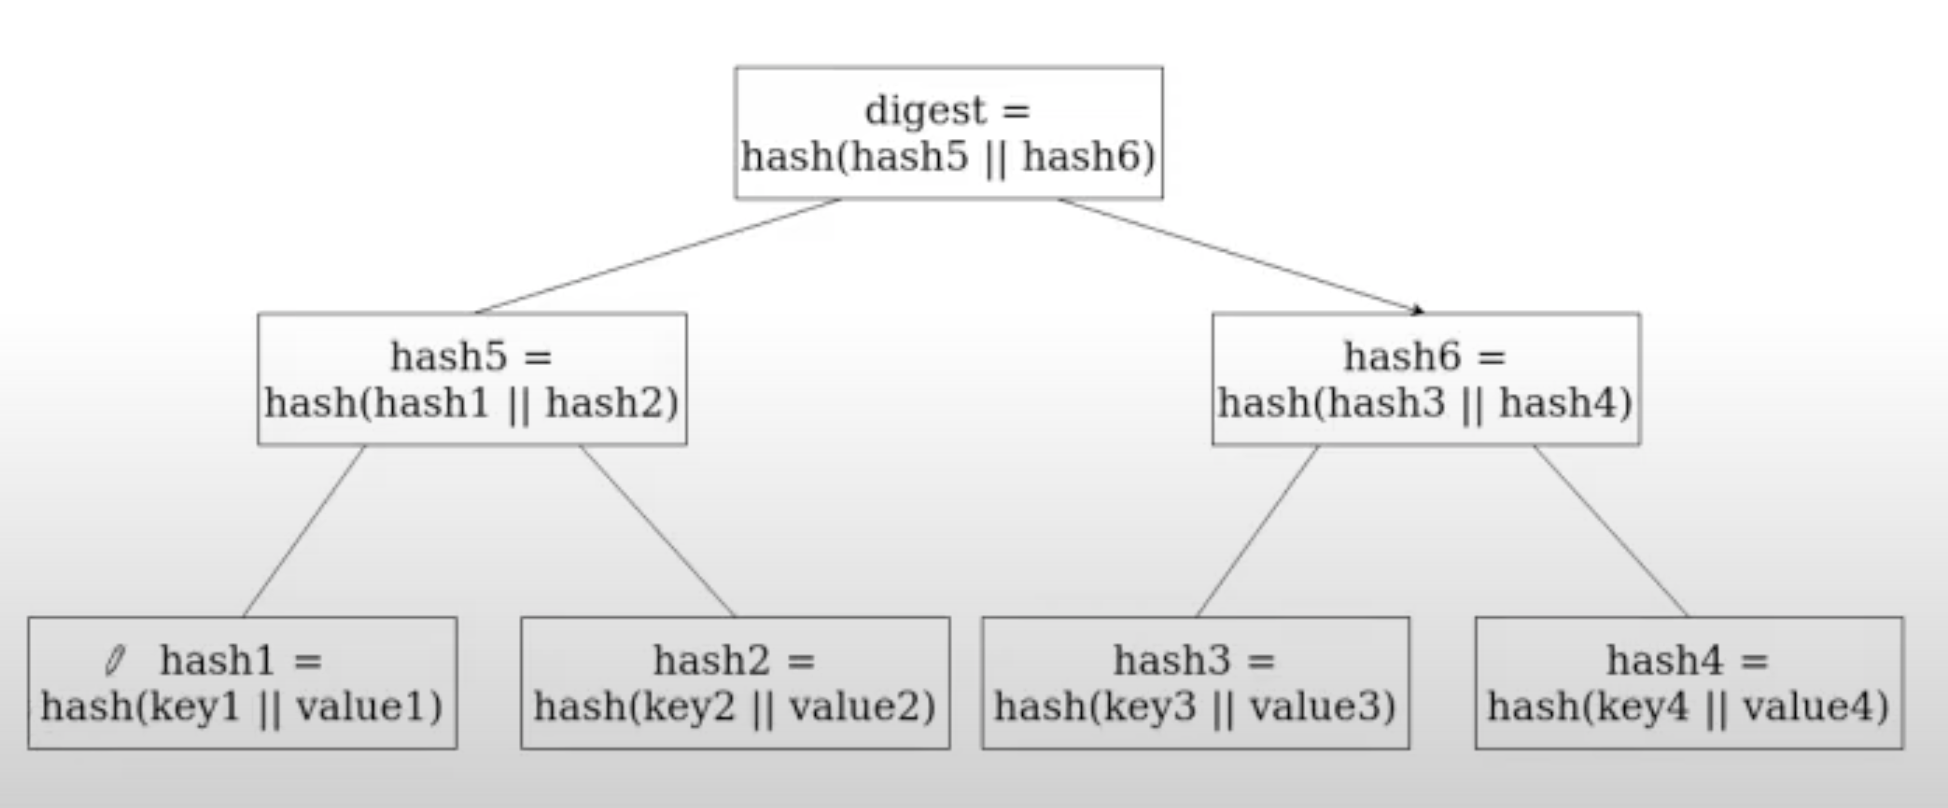
\includegraphics[scale = 0.5]{../assets/17.png}
        \caption{Дерево Меркла}
    \end{figure}
    \item использование деревьев Мёркла - чтобы быстро понять синхронизированы ли версии, сравним корни деревьев Мёркла, построенных на каждой из реплик, если они равны, считаем что версии синхронизированны, если не равны, смотрим в каком из детей не равны хеши и рекурсивно спускаемся до листьев, пока не найдём различающиеся значения.
\end{itemize}
\begin{definition}
  Sloppy Quorum
\end{definition}
  \begin{itemize}
    \item Если читаем с единственной реплики, велик шанс прочесть устаревшее значение (например, она может быть медленная).
    \item Будем читать с $R$ реплик и брать самое свежее среди них значение, так уменьшается вероятность прочитать устаревшее значение, если прочитали несколько параллельных версий - решаем конфликт.
    \item Если пишем на одну реплику, она может быть медленнее, рискуем потерять Durability при ее падении (которое нельзя восстановить)
    \item Аналогично при записи, будем писать на $W$ реплик, так запись быстрее отреплицируется на копии. Клиенту сообщаем, что запись удалась только после записи на все из этих $W$ реплик. Также можем эти $W$ записей транзакционно \\
    \item $N$ - количество узлов в кластере, тогда: \\
        $R + W > N$ - каждая подтверждённая запись будет прочитана \\
        $R + W <= N$ - улучшается Durability записи, уменьшается вероятность прочитать старое значение, но можем не прочесть сделанную запись.
  \end{itemize}
  \begin{definition}
    Hinted Handoff
  \end{definition}
  \begin{itemize}
    \item Иногда, из-за недоступности, мы не можем сделать запись на $W$ узлов, тогда сделаем запись на узлы которые не должны хранить наши данные (например, узлы, являющиеся репликами другой партиции). \\
    эти узлы знают, что они хранят записи, не принадлежащие им, когда-нибудь, они отреплицируют эти данные на нужные узлы после их поднятия.
  \end{itemize}
